\documentclass[tikz]{standalone}

\usetikzlibrary{calc,positioning,shapes,positioning,intersections,quotes,decorations.markings}
\usepackage{amsfonts,amsmath,amsthm,amssymb,mathtools,stmaryrd,mathrsfs}

\begin{document}
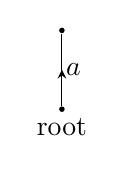
\begin{tikzpicture}[>=stealth,decoration={
				markings,
				mark=at position 0.5 with {\arrow{>}}}
	]

	\node[circle,fill=black,inner sep=0pt,minimum size=2pt] (n0) at (0,0){}node[below]{root} ;

	\node[circle,fill=black,inner sep=0pt,minimum size=2pt] (n1) at (0,1) {};
  
	\draw[postaction={decorate}] (n0) --node[right=-2pt]{$a$} (n1);

\end{tikzpicture}
\end{document}
